% Graphic for TeX using PGF
% Title: /home/marta/Diagrama3.dia
% Creator: Dia v0.97.3
% CreationDate: Thu Sep  7 23:36:28 2017
% For: marta
% \usepackage{tikz}
% The following commands are not supported in PSTricks at present
% We define them conditionally, so when they are implemented,
% this pgf file will use them.
\ifx\du\undefined
  \newlength{\du}
\fi
\setlength{\du}{15\unitlength}
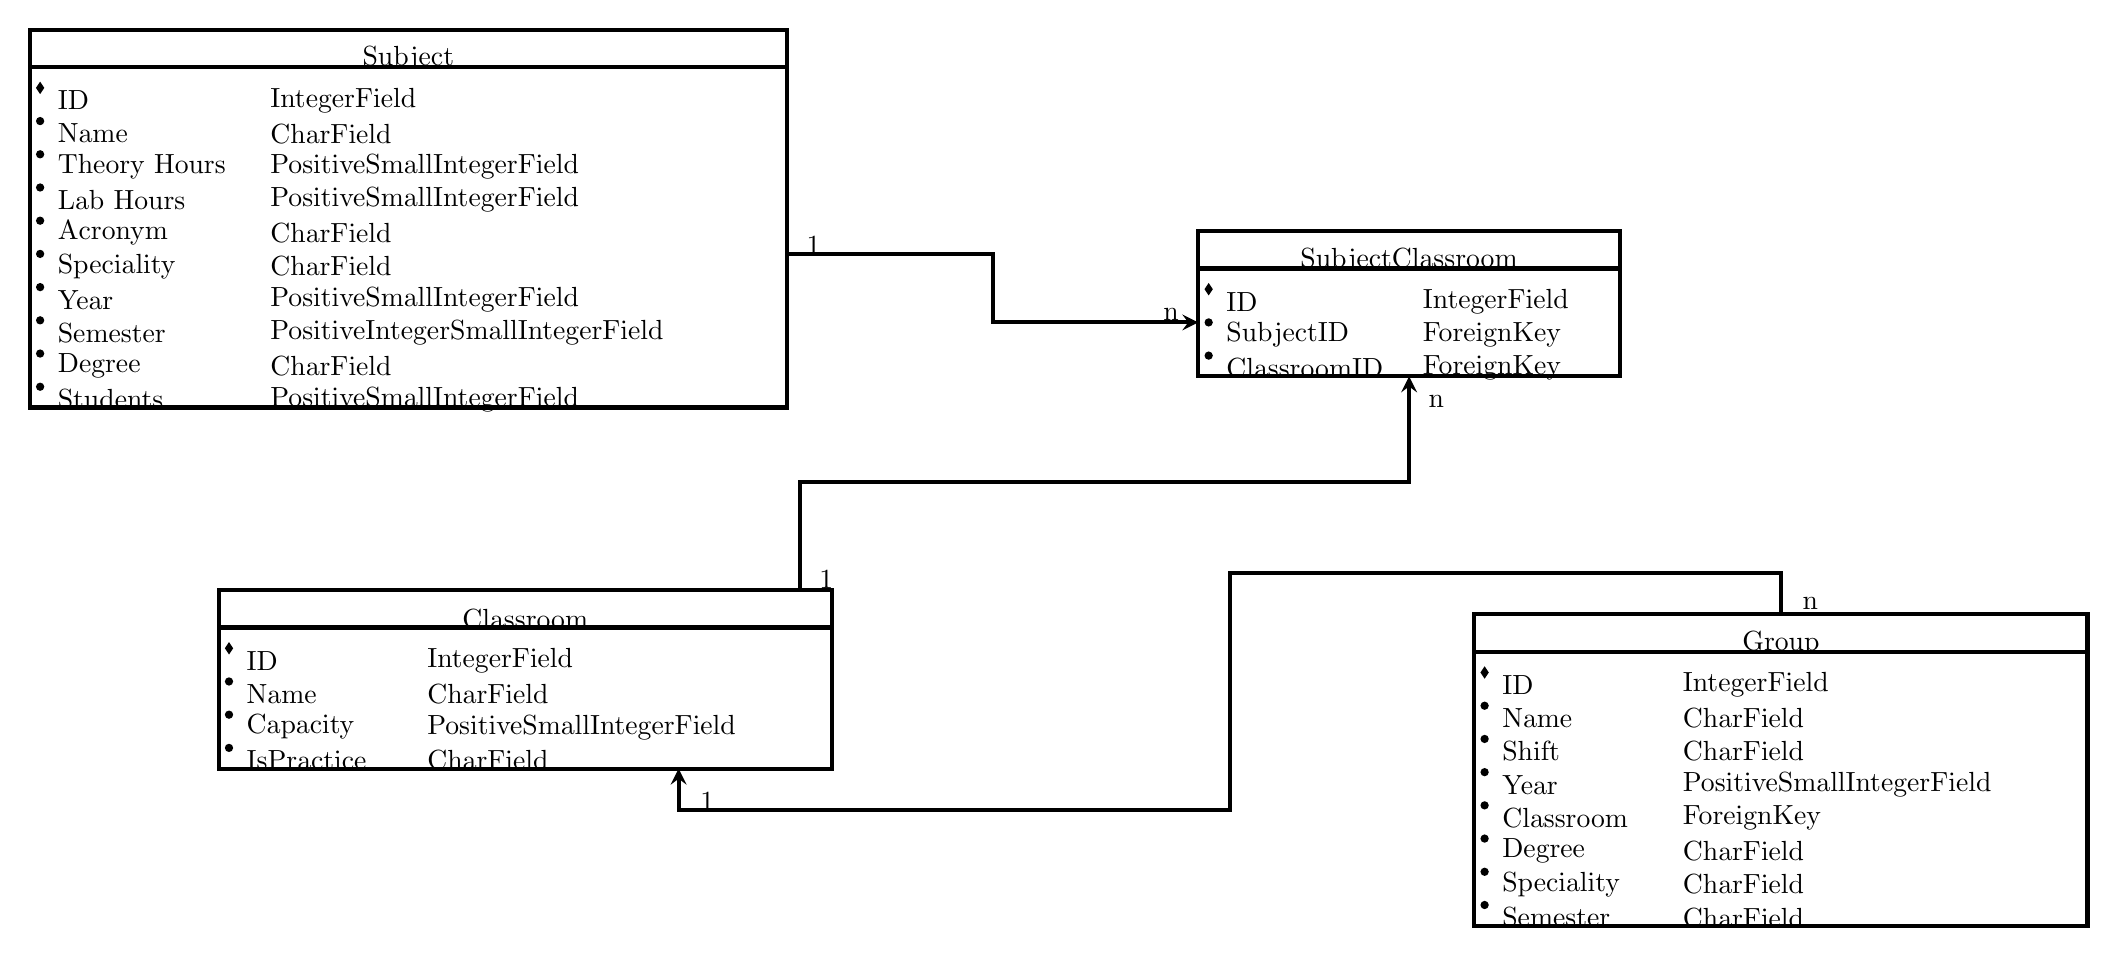
\begin{tikzpicture}
\pgftransformxscale{1.000000}
\pgftransformyscale{-1.000000}
\definecolor{dialinecolor}{rgb}{0.000000, 0.000000, 0.000000}
\pgfsetstrokecolor{dialinecolor}
\definecolor{dialinecolor}{rgb}{1.000000, 1.000000, 1.000000}
\pgfsetfillcolor{dialinecolor}
\pgfsetlinewidth{0.100000\du}
\pgfsetdash{}{0pt}
\definecolor{dialinecolor}{rgb}{1.000000, 1.000000, 1.000000}
\pgfsetfillcolor{dialinecolor}
\fill (3.300000\du,3.600000\du)--(3.300000\du,4.500000\du)--(21.540000\du,4.500000\du)--(21.540000\du,3.600000\du)--cycle;
\definecolor{dialinecolor}{rgb}{0.000000, 0.000000, 0.000000}
\pgfsetstrokecolor{dialinecolor}
\draw (3.300000\du,3.600000\du)--(3.300000\du,4.500000\du)--(21.540000\du,4.500000\du)--(21.540000\du,3.600000\du)--cycle;
% setfont left to latex
\definecolor{dialinecolor}{rgb}{0.000000, 0.000000, 0.000000}
\pgfsetstrokecolor{dialinecolor}
\node at (12.420000\du,4.300000\du){Subject};
\definecolor{dialinecolor}{rgb}{1.000000, 1.000000, 1.000000}
\pgfsetfillcolor{dialinecolor}
\fill (3.300000\du,4.500000\du)--(3.300000\du,12.700000\du)--(21.540000\du,12.700000\du)--(21.540000\du,4.500000\du)--cycle;
\definecolor{dialinecolor}{rgb}{0.000000, 0.000000, 0.000000}
\pgfsetstrokecolor{dialinecolor}
\draw (3.300000\du,4.500000\du)--(3.300000\du,12.700000\du)--(21.540000\du,12.700000\du)--(21.540000\du,4.500000\du)--cycle;
% setfont left to latex
\pgfsetlinewidth{0.010000\du}
\pgfsetmiterjoin
\definecolor{dialinecolor}{rgb}{0.000000, 0.000000, 0.000000}
\pgfsetfillcolor{dialinecolor}
\fill (3.450000\du,5.000000\du)--(3.550000\du,5.150000\du)--(3.650000\du,5.000000\du)--(3.550000\du,4.850000\du)--cycle;
\definecolor{dialinecolor}{rgb}{0.000000, 0.000000, 0.000000}
\pgfsetstrokecolor{dialinecolor}
\node[anchor=west] at (3.750000\du,5.300000\du){ID};
\definecolor{dialinecolor}{rgb}{0.000000, 0.000000, 0.000000}
\pgfsetstrokecolor{dialinecolor}
\node[anchor=west] at (8.870000\du,5.300000\du){IntegerField};
% setfont left to latex
\pgfsetlinewidth{0.010000\du}
\definecolor{dialinecolor}{rgb}{0.000000, 0.000000, 0.000000}
\pgfsetfillcolor{dialinecolor}
\pgfpathellipse{\pgfpoint{3.550000\du}{5.800000\du}}{\pgfpoint{0.100000\du}{0\du}}{\pgfpoint{0\du}{0.100000\du}}
\pgfusepath{fill}
\definecolor{dialinecolor}{rgb}{0.000000, 0.000000, 0.000000}
\pgfsetstrokecolor{dialinecolor}
\node[anchor=west] at (3.750000\du,6.100000\du){Name};
\definecolor{dialinecolor}{rgb}{0.000000, 0.000000, 0.000000}
\pgfsetstrokecolor{dialinecolor}
\node[anchor=west] at (8.870000\du,6.100000\du){CharField};
% setfont left to latex
\pgfsetlinewidth{0.010000\du}
\definecolor{dialinecolor}{rgb}{0.000000, 0.000000, 0.000000}
\pgfsetfillcolor{dialinecolor}
\pgfpathellipse{\pgfpoint{3.550000\du}{6.600000\du}}{\pgfpoint{0.100000\du}{0\du}}{\pgfpoint{0\du}{0.100000\du}}
\pgfusepath{fill}
\definecolor{dialinecolor}{rgb}{0.000000, 0.000000, 0.000000}
\pgfsetstrokecolor{dialinecolor}
\node[anchor=west] at (3.750000\du,6.900000\du){Theory Hours};
\definecolor{dialinecolor}{rgb}{0.000000, 0.000000, 0.000000}
\pgfsetstrokecolor{dialinecolor}
\node[anchor=west] at (8.870000\du,6.900000\du){PositiveSmallIntegerField};
% setfont left to latex
\pgfsetlinewidth{0.010000\du}
\definecolor{dialinecolor}{rgb}{0.000000, 0.000000, 0.000000}
\pgfsetfillcolor{dialinecolor}
\pgfpathellipse{\pgfpoint{3.550000\du}{7.400000\du}}{\pgfpoint{0.100000\du}{0\du}}{\pgfpoint{0\du}{0.100000\du}}
\pgfusepath{fill}
\definecolor{dialinecolor}{rgb}{0.000000, 0.000000, 0.000000}
\pgfsetstrokecolor{dialinecolor}
\node[anchor=west] at (3.750000\du,7.700000\du){Lab Hours};
\definecolor{dialinecolor}{rgb}{0.000000, 0.000000, 0.000000}
\pgfsetstrokecolor{dialinecolor}
\node[anchor=west] at (8.870000\du,7.700000\du){PositiveSmallIntegerField};
% setfont left to latex
\pgfsetlinewidth{0.010000\du}
\definecolor{dialinecolor}{rgb}{0.000000, 0.000000, 0.000000}
\pgfsetfillcolor{dialinecolor}
\pgfpathellipse{\pgfpoint{3.550000\du}{8.200000\du}}{\pgfpoint{0.100000\du}{0\du}}{\pgfpoint{0\du}{0.100000\du}}
\pgfusepath{fill}
\definecolor{dialinecolor}{rgb}{0.000000, 0.000000, 0.000000}
\pgfsetstrokecolor{dialinecolor}
\node[anchor=west] at (3.750000\du,8.500000\du){Acronym};
\definecolor{dialinecolor}{rgb}{0.000000, 0.000000, 0.000000}
\pgfsetstrokecolor{dialinecolor}
\node[anchor=west] at (8.870000\du,8.500000\du){CharField};
% setfont left to latex
\pgfsetlinewidth{0.010000\du}
\definecolor{dialinecolor}{rgb}{0.000000, 0.000000, 0.000000}
\pgfsetfillcolor{dialinecolor}
\pgfpathellipse{\pgfpoint{3.550000\du}{9.000000\du}}{\pgfpoint{0.100000\du}{0\du}}{\pgfpoint{0\du}{0.100000\du}}
\pgfusepath{fill}
\definecolor{dialinecolor}{rgb}{0.000000, 0.000000, 0.000000}
\pgfsetstrokecolor{dialinecolor}
\node[anchor=west] at (3.750000\du,9.300000\du){Speciality};
\definecolor{dialinecolor}{rgb}{0.000000, 0.000000, 0.000000}
\pgfsetstrokecolor{dialinecolor}
\node[anchor=west] at (8.870000\du,9.300000\du){CharField};
% setfont left to latex
\pgfsetlinewidth{0.010000\du}
\definecolor{dialinecolor}{rgb}{0.000000, 0.000000, 0.000000}
\pgfsetfillcolor{dialinecolor}
\pgfpathellipse{\pgfpoint{3.550000\du}{9.800000\du}}{\pgfpoint{0.100000\du}{0\du}}{\pgfpoint{0\du}{0.100000\du}}
\pgfusepath{fill}
\definecolor{dialinecolor}{rgb}{0.000000, 0.000000, 0.000000}
\pgfsetstrokecolor{dialinecolor}
\node[anchor=west] at (3.750000\du,10.100000\du){Year};
\definecolor{dialinecolor}{rgb}{0.000000, 0.000000, 0.000000}
\pgfsetstrokecolor{dialinecolor}
\node[anchor=west] at (8.870000\du,10.100000\du){PositiveSmallIntegerField};
% setfont left to latex
\pgfsetlinewidth{0.010000\du}
\definecolor{dialinecolor}{rgb}{0.000000, 0.000000, 0.000000}
\pgfsetfillcolor{dialinecolor}
\pgfpathellipse{\pgfpoint{3.550000\du}{10.600000\du}}{\pgfpoint{0.100000\du}{0\du}}{\pgfpoint{0\du}{0.100000\du}}
\pgfusepath{fill}
\definecolor{dialinecolor}{rgb}{0.000000, 0.000000, 0.000000}
\pgfsetstrokecolor{dialinecolor}
\node[anchor=west] at (3.750000\du,10.900000\du){Semester};
\definecolor{dialinecolor}{rgb}{0.000000, 0.000000, 0.000000}
\pgfsetstrokecolor{dialinecolor}
\node[anchor=west] at (8.870000\du,10.900000\du){PositiveIntegerSmallIntegerField};
% setfont left to latex
\pgfsetlinewidth{0.010000\du}
\definecolor{dialinecolor}{rgb}{0.000000, 0.000000, 0.000000}
\pgfsetfillcolor{dialinecolor}
\pgfpathellipse{\pgfpoint{3.550000\du}{11.400000\du}}{\pgfpoint{0.100000\du}{0\du}}{\pgfpoint{0\du}{0.100000\du}}
\pgfusepath{fill}
\definecolor{dialinecolor}{rgb}{0.000000, 0.000000, 0.000000}
\pgfsetstrokecolor{dialinecolor}
\node[anchor=west] at (3.750000\du,11.700000\du){Degree};
\definecolor{dialinecolor}{rgb}{0.000000, 0.000000, 0.000000}
\pgfsetstrokecolor{dialinecolor}
\node[anchor=west] at (8.870000\du,11.700000\du){CharField};
% setfont left to latex
\pgfsetlinewidth{0.010000\du}
\definecolor{dialinecolor}{rgb}{0.000000, 0.000000, 0.000000}
\pgfsetfillcolor{dialinecolor}
\pgfpathellipse{\pgfpoint{3.550000\du}{12.200000\du}}{\pgfpoint{0.100000\du}{0\du}}{\pgfpoint{0\du}{0.100000\du}}
\pgfusepath{fill}
\definecolor{dialinecolor}{rgb}{0.000000, 0.000000, 0.000000}
\pgfsetstrokecolor{dialinecolor}
\node[anchor=west] at (3.750000\du,12.500000\du){Students};
\definecolor{dialinecolor}{rgb}{0.000000, 0.000000, 0.000000}
\pgfsetstrokecolor{dialinecolor}
\node[anchor=west] at (8.870000\du,12.500000\du){PositiveSmallIntegerField};
\pgfsetlinewidth{0.100000\du}
\pgfsetdash{}{0pt}
\definecolor{dialinecolor}{rgb}{1.000000, 1.000000, 1.000000}
\pgfsetfillcolor{dialinecolor}
\fill (7.850000\du,17.100000\du)--(7.850000\du,18.000000\du)--(22.625000\du,18.000000\du)--(22.625000\du,17.100000\du)--cycle;
\definecolor{dialinecolor}{rgb}{0.000000, 0.000000, 0.000000}
\pgfsetstrokecolor{dialinecolor}
\draw (7.850000\du,17.100000\du)--(7.850000\du,18.000000\du)--(22.625000\du,18.000000\du)--(22.625000\du,17.100000\du)--cycle;
% setfont left to latex
\definecolor{dialinecolor}{rgb}{0.000000, 0.000000, 0.000000}
\pgfsetstrokecolor{dialinecolor}
\node at (15.237500\du,17.800000\du){Classroom};
\definecolor{dialinecolor}{rgb}{1.000000, 1.000000, 1.000000}
\pgfsetfillcolor{dialinecolor}
\fill (7.850000\du,18.000000\du)--(7.850000\du,21.400000\du)--(22.625000\du,21.400000\du)--(22.625000\du,18.000000\du)--cycle;
\definecolor{dialinecolor}{rgb}{0.000000, 0.000000, 0.000000}
\pgfsetstrokecolor{dialinecolor}
\draw (7.850000\du,18.000000\du)--(7.850000\du,21.400000\du)--(22.625000\du,21.400000\du)--(22.625000\du,18.000000\du)--cycle;
% setfont left to latex
\pgfsetlinewidth{0.010000\du}
\pgfsetmiterjoin
\definecolor{dialinecolor}{rgb}{0.000000, 0.000000, 0.000000}
\pgfsetfillcolor{dialinecolor}
\fill (8.000000\du,18.500000\du)--(8.100000\du,18.650000\du)--(8.200000\du,18.500000\du)--(8.100000\du,18.350000\du)--cycle;
\definecolor{dialinecolor}{rgb}{0.000000, 0.000000, 0.000000}
\pgfsetstrokecolor{dialinecolor}
\node[anchor=west] at (8.300000\du,18.800000\du){ID};
\definecolor{dialinecolor}{rgb}{0.000000, 0.000000, 0.000000}
\pgfsetstrokecolor{dialinecolor}
\node[anchor=west] at (12.650000\du,18.800000\du){IntegerField};
% setfont left to latex
\pgfsetlinewidth{0.010000\du}
\definecolor{dialinecolor}{rgb}{0.000000, 0.000000, 0.000000}
\pgfsetfillcolor{dialinecolor}
\pgfpathellipse{\pgfpoint{8.100000\du}{19.300000\du}}{\pgfpoint{0.100000\du}{0\du}}{\pgfpoint{0\du}{0.100000\du}}
\pgfusepath{fill}
\definecolor{dialinecolor}{rgb}{0.000000, 0.000000, 0.000000}
\pgfsetstrokecolor{dialinecolor}
\node[anchor=west] at (8.300000\du,19.600000\du){Name};
\definecolor{dialinecolor}{rgb}{0.000000, 0.000000, 0.000000}
\pgfsetstrokecolor{dialinecolor}
\node[anchor=west] at (12.650000\du,19.600000\du){CharField};
% setfont left to latex
\pgfsetlinewidth{0.010000\du}
\definecolor{dialinecolor}{rgb}{0.000000, 0.000000, 0.000000}
\pgfsetfillcolor{dialinecolor}
\pgfpathellipse{\pgfpoint{8.100000\du}{20.100000\du}}{\pgfpoint{0.100000\du}{0\du}}{\pgfpoint{0\du}{0.100000\du}}
\pgfusepath{fill}
\definecolor{dialinecolor}{rgb}{0.000000, 0.000000, 0.000000}
\pgfsetstrokecolor{dialinecolor}
\node[anchor=west] at (8.300000\du,20.400000\du){Capacity};
\definecolor{dialinecolor}{rgb}{0.000000, 0.000000, 0.000000}
\pgfsetstrokecolor{dialinecolor}
\node[anchor=west] at (12.650000\du,20.400000\du){PositiveSmallIntegerField};
% setfont left to latex
\pgfsetlinewidth{0.010000\du}
\definecolor{dialinecolor}{rgb}{0.000000, 0.000000, 0.000000}
\pgfsetfillcolor{dialinecolor}
\pgfpathellipse{\pgfpoint{8.100000\du}{20.900000\du}}{\pgfpoint{0.100000\du}{0\du}}{\pgfpoint{0\du}{0.100000\du}}
\pgfusepath{fill}
\definecolor{dialinecolor}{rgb}{0.000000, 0.000000, 0.000000}
\pgfsetstrokecolor{dialinecolor}
\node[anchor=west] at (8.300000\du,21.200000\du){IsPractice};
\definecolor{dialinecolor}{rgb}{0.000000, 0.000000, 0.000000}
\pgfsetstrokecolor{dialinecolor}
\node[anchor=west] at (12.650000\du,21.200000\du){CharField};
\pgfsetlinewidth{0.100000\du}
\pgfsetdash{}{0pt}
\definecolor{dialinecolor}{rgb}{1.000000, 1.000000, 1.000000}
\pgfsetfillcolor{dialinecolor}
\fill (38.097224\du,17.684124\du)--(38.097224\du,18.584124\du)--(52.872224\du,18.584124\du)--(52.872224\du,17.684124\du)--cycle;
\definecolor{dialinecolor}{rgb}{0.000000, 0.000000, 0.000000}
\pgfsetstrokecolor{dialinecolor}
\draw (38.097224\du,17.684124\du)--(38.097224\du,18.584124\du)--(52.872224\du,18.584124\du)--(52.872224\du,17.684124\du)--cycle;
% setfont left to latex
\definecolor{dialinecolor}{rgb}{0.000000, 0.000000, 0.000000}
\pgfsetstrokecolor{dialinecolor}
\node at (45.484724\du,18.384124\du){Group};
\definecolor{dialinecolor}{rgb}{1.000000, 1.000000, 1.000000}
\pgfsetfillcolor{dialinecolor}
\fill (38.097224\du,18.584124\du)--(38.097224\du,25.184124\du)--(52.872224\du,25.184124\du)--(52.872224\du,18.584124\du)--cycle;
\definecolor{dialinecolor}{rgb}{0.000000, 0.000000, 0.000000}
\pgfsetstrokecolor{dialinecolor}
\draw (38.097224\du,18.584124\du)--(38.097224\du,25.184124\du)--(52.872224\du,25.184124\du)--(52.872224\du,18.584124\du)--cycle;
% setfont left to latex
\pgfsetlinewidth{0.010000\du}
\pgfsetmiterjoin
\definecolor{dialinecolor}{rgb}{0.000000, 0.000000, 0.000000}
\pgfsetfillcolor{dialinecolor}
\fill (38.247224\du,19.084124\du)--(38.347224\du,19.234124\du)--(38.447224\du,19.084124\du)--(38.347224\du,18.934124\du)--cycle;
\definecolor{dialinecolor}{rgb}{0.000000, 0.000000, 0.000000}
\pgfsetstrokecolor{dialinecolor}
\node[anchor=west] at (38.547224\du,19.384124\du){ID};
\definecolor{dialinecolor}{rgb}{0.000000, 0.000000, 0.000000}
\pgfsetstrokecolor{dialinecolor}
\node[anchor=west] at (42.897224\du,19.384124\du){IntegerField};
% setfont left to latex
\pgfsetlinewidth{0.010000\du}
\definecolor{dialinecolor}{rgb}{0.000000, 0.000000, 0.000000}
\pgfsetfillcolor{dialinecolor}
\pgfpathellipse{\pgfpoint{38.347224\du}{19.884124\du}}{\pgfpoint{0.100000\du}{0\du}}{\pgfpoint{0\du}{0.100000\du}}
\pgfusepath{fill}
\definecolor{dialinecolor}{rgb}{0.000000, 0.000000, 0.000000}
\pgfsetstrokecolor{dialinecolor}
\node[anchor=west] at (38.547224\du,20.184124\du){Name};
\definecolor{dialinecolor}{rgb}{0.000000, 0.000000, 0.000000}
\pgfsetstrokecolor{dialinecolor}
\node[anchor=west] at (42.897224\du,20.184124\du){CharField};
% setfont left to latex
\pgfsetlinewidth{0.010000\du}
\definecolor{dialinecolor}{rgb}{0.000000, 0.000000, 0.000000}
\pgfsetfillcolor{dialinecolor}
\pgfpathellipse{\pgfpoint{38.347224\du}{20.684124\du}}{\pgfpoint{0.100000\du}{0\du}}{\pgfpoint{0\du}{0.100000\du}}
\pgfusepath{fill}
\definecolor{dialinecolor}{rgb}{0.000000, 0.000000, 0.000000}
\pgfsetstrokecolor{dialinecolor}
\node[anchor=west] at (38.547224\du,20.984124\du){Shift};
\definecolor{dialinecolor}{rgb}{0.000000, 0.000000, 0.000000}
\pgfsetstrokecolor{dialinecolor}
\node[anchor=west] at (42.897224\du,20.984124\du){CharField};
% setfont left to latex
\pgfsetlinewidth{0.010000\du}
\definecolor{dialinecolor}{rgb}{0.000000, 0.000000, 0.000000}
\pgfsetfillcolor{dialinecolor}
\pgfpathellipse{\pgfpoint{38.347224\du}{21.484124\du}}{\pgfpoint{0.100000\du}{0\du}}{\pgfpoint{0\du}{0.100000\du}}
\pgfusepath{fill}
\definecolor{dialinecolor}{rgb}{0.000000, 0.000000, 0.000000}
\pgfsetstrokecolor{dialinecolor}
\node[anchor=west] at (38.547224\du,21.784124\du){Year};
\definecolor{dialinecolor}{rgb}{0.000000, 0.000000, 0.000000}
\pgfsetstrokecolor{dialinecolor}
\node[anchor=west] at (42.897224\du,21.784124\du){PositiveSmallIntegerField};
% setfont left to latex
\pgfsetlinewidth{0.010000\du}
\definecolor{dialinecolor}{rgb}{0.000000, 0.000000, 0.000000}
\pgfsetfillcolor{dialinecolor}
\pgfpathellipse{\pgfpoint{38.347224\du}{22.284124\du}}{\pgfpoint{0.100000\du}{0\du}}{\pgfpoint{0\du}{0.100000\du}}
\pgfusepath{fill}
\definecolor{dialinecolor}{rgb}{0.000000, 0.000000, 0.000000}
\pgfsetstrokecolor{dialinecolor}
\node[anchor=west] at (38.547224\du,22.584124\du){Classroom};
\definecolor{dialinecolor}{rgb}{0.000000, 0.000000, 0.000000}
\pgfsetstrokecolor{dialinecolor}
\node[anchor=west] at (42.897224\du,22.584124\du){ForeignKey};
% setfont left to latex
\pgfsetlinewidth{0.010000\du}
\definecolor{dialinecolor}{rgb}{0.000000, 0.000000, 0.000000}
\pgfsetfillcolor{dialinecolor}
\pgfpathellipse{\pgfpoint{38.347224\du}{23.084124\du}}{\pgfpoint{0.100000\du}{0\du}}{\pgfpoint{0\du}{0.100000\du}}
\pgfusepath{fill}
\definecolor{dialinecolor}{rgb}{0.000000, 0.000000, 0.000000}
\pgfsetstrokecolor{dialinecolor}
\node[anchor=west] at (38.547224\du,23.384124\du){Degree};
\definecolor{dialinecolor}{rgb}{0.000000, 0.000000, 0.000000}
\pgfsetstrokecolor{dialinecolor}
\node[anchor=west] at (42.897224\du,23.384124\du){CharField};
% setfont left to latex
\pgfsetlinewidth{0.010000\du}
\definecolor{dialinecolor}{rgb}{0.000000, 0.000000, 0.000000}
\pgfsetfillcolor{dialinecolor}
\pgfpathellipse{\pgfpoint{38.347224\du}{23.884124\du}}{\pgfpoint{0.100000\du}{0\du}}{\pgfpoint{0\du}{0.100000\du}}
\pgfusepath{fill}
\definecolor{dialinecolor}{rgb}{0.000000, 0.000000, 0.000000}
\pgfsetstrokecolor{dialinecolor}
\node[anchor=west] at (38.547224\du,24.184124\du){Speciality};
\definecolor{dialinecolor}{rgb}{0.000000, 0.000000, 0.000000}
\pgfsetstrokecolor{dialinecolor}
\node[anchor=west] at (42.897224\du,24.184124\du){CharField};
% setfont left to latex
\pgfsetlinewidth{0.010000\du}
\definecolor{dialinecolor}{rgb}{0.000000, 0.000000, 0.000000}
\pgfsetfillcolor{dialinecolor}
\pgfpathellipse{\pgfpoint{38.347224\du}{24.684124\du}}{\pgfpoint{0.100000\du}{0\du}}{\pgfpoint{0\du}{0.100000\du}}
\pgfusepath{fill}
\definecolor{dialinecolor}{rgb}{0.000000, 0.000000, 0.000000}
\pgfsetstrokecolor{dialinecolor}
\node[anchor=west] at (38.547224\du,24.984124\du){Semester};
\definecolor{dialinecolor}{rgb}{0.000000, 0.000000, 0.000000}
\pgfsetstrokecolor{dialinecolor}
\node[anchor=west] at (42.897224\du,24.984124\du){CharField};
\pgfsetlinewidth{0.100000\du}
\pgfsetdash{}{0pt}
\pgfsetdash{}{0pt}
\pgfsetmiterjoin
\pgfsetbuttcap
{
\definecolor{dialinecolor}{rgb}{0.000000, 0.000000, 0.000000}
\pgfsetfillcolor{dialinecolor}
% was here!!!
\pgfsetarrowsend{stealth}
{\pgfsetcornersarced{\pgfpoint{0.000000\du}{0.000000\du}}\definecolor{dialinecolor}{rgb}{0.000000, 0.000000, 0.000000}
\pgfsetstrokecolor{dialinecolor}
\draw (45.484724\du,17.684124\du)--(45.484724\du,16.684124\du)--(32.207987\du,16.684124\du)--(32.207987\du,22.400000\du)--(18.931250\du,22.400000\du)--(18.931250\du,21.400000\du);
}}
% setfont left to latex
\definecolor{dialinecolor}{rgb}{0.000000, 0.000000, 0.000000}
\pgfsetstrokecolor{dialinecolor}
\node[anchor=west] at (45.734724\du,17.434124\du){n};
\definecolor{dialinecolor}{rgb}{0.000000, 0.000000, 0.000000}
\pgfsetstrokecolor{dialinecolor}
\node[anchor=west] at (19.181250\du,22.200000\du){1};
\pgfsetlinewidth{0.100000\du}
\pgfsetdash{}{0pt}
\definecolor{dialinecolor}{rgb}{1.000000, 1.000000, 1.000000}
\pgfsetfillcolor{dialinecolor}
\fill (31.449993\du,8.449997\du)--(31.449993\du,9.349997\du)--(41.604993\du,9.349997\du)--(41.604993\du,8.449997\du)--cycle;
\definecolor{dialinecolor}{rgb}{0.000000, 0.000000, 0.000000}
\pgfsetstrokecolor{dialinecolor}
\draw (31.449993\du,8.449997\du)--(31.449993\du,9.349997\du)--(41.604993\du,9.349997\du)--(41.604993\du,8.449997\du)--cycle;
% setfont left to latex
\definecolor{dialinecolor}{rgb}{0.000000, 0.000000, 0.000000}
\pgfsetstrokecolor{dialinecolor}
\node at (36.527493\du,9.149997\du){SubjectClassroom};
\definecolor{dialinecolor}{rgb}{1.000000, 1.000000, 1.000000}
\pgfsetfillcolor{dialinecolor}
\fill (31.449993\du,9.349997\du)--(31.449993\du,11.949997\du)--(41.604993\du,11.949997\du)--(41.604993\du,9.349997\du)--cycle;
\definecolor{dialinecolor}{rgb}{0.000000, 0.000000, 0.000000}
\pgfsetstrokecolor{dialinecolor}
\draw (31.449993\du,9.349997\du)--(31.449993\du,11.949997\du)--(41.604993\du,11.949997\du)--(41.604993\du,9.349997\du)--cycle;
% setfont left to latex
\pgfsetlinewidth{0.010000\du}
\pgfsetmiterjoin
\definecolor{dialinecolor}{rgb}{0.000000, 0.000000, 0.000000}
\pgfsetfillcolor{dialinecolor}
\fill (31.599993\du,9.849997\du)--(31.699993\du,9.999997\du)--(31.799993\du,9.849997\du)--(31.699993\du,9.699997\du)--cycle;
\definecolor{dialinecolor}{rgb}{0.000000, 0.000000, 0.000000}
\pgfsetstrokecolor{dialinecolor}
\node[anchor=west] at (31.899993\du,10.149997\du){ID};
\definecolor{dialinecolor}{rgb}{0.000000, 0.000000, 0.000000}
\pgfsetstrokecolor{dialinecolor}
\node[anchor=west] at (36.634993\du,10.149997\du){IntegerField};
% setfont left to latex
\pgfsetlinewidth{0.010000\du}
\definecolor{dialinecolor}{rgb}{0.000000, 0.000000, 0.000000}
\pgfsetfillcolor{dialinecolor}
\pgfpathellipse{\pgfpoint{31.699993\du}{10.649997\du}}{\pgfpoint{0.100000\du}{0\du}}{\pgfpoint{0\du}{0.100000\du}}
\pgfusepath{fill}
\definecolor{dialinecolor}{rgb}{0.000000, 0.000000, 0.000000}
\pgfsetstrokecolor{dialinecolor}
\node[anchor=west] at (31.899993\du,10.949997\du){SubjectID};
\definecolor{dialinecolor}{rgb}{0.000000, 0.000000, 0.000000}
\pgfsetstrokecolor{dialinecolor}
\node[anchor=west] at (36.634993\du,10.949997\du){ForeignKey};
% setfont left to latex
\pgfsetlinewidth{0.010000\du}
\definecolor{dialinecolor}{rgb}{0.000000, 0.000000, 0.000000}
\pgfsetfillcolor{dialinecolor}
\pgfpathellipse{\pgfpoint{31.699993\du}{11.449997\du}}{\pgfpoint{0.100000\du}{0\du}}{\pgfpoint{0\du}{0.100000\du}}
\pgfusepath{fill}
\definecolor{dialinecolor}{rgb}{0.000000, 0.000000, 0.000000}
\pgfsetstrokecolor{dialinecolor}
\node[anchor=west] at (31.899993\du,11.749997\du){ClassroomID};
\definecolor{dialinecolor}{rgb}{0.000000, 0.000000, 0.000000}
\pgfsetstrokecolor{dialinecolor}
\node[anchor=west] at (36.634993\du,11.749997\du){ForeignKey};
\pgfsetlinewidth{0.100000\du}
\pgfsetdash{}{0pt}
\pgfsetdash{}{0pt}
\pgfsetmiterjoin
\pgfsetbuttcap
{
\definecolor{dialinecolor}{rgb}{0.000000, 0.000000, 0.000000}
\pgfsetfillcolor{dialinecolor}
% was here!!!
\pgfsetarrowsend{stealth}
{\pgfsetcornersarced{\pgfpoint{0.000000\du}{0.000000\du}}\definecolor{dialinecolor}{rgb}{0.000000, 0.000000, 0.000000}
\pgfsetstrokecolor{dialinecolor}
\draw (21.540000\du,9.000000\du)--(26.494997\du,9.000000\du)--(26.494997\du,10.649997\du)--(31.449993\du,10.649997\du);
}}
% setfont left to latex
\definecolor{dialinecolor}{rgb}{0.000000, 0.000000, 0.000000}
\pgfsetstrokecolor{dialinecolor}
\node[anchor=west] at (21.740000\du,8.800000\du){1};
\definecolor{dialinecolor}{rgb}{0.000000, 0.000000, 0.000000}
\pgfsetstrokecolor{dialinecolor}
\node[anchor=east] at (31.249993\du,10.449997\du){n};
\pgfsetlinewidth{0.100000\du}
\pgfsetdash{}{0pt}
\pgfsetdash{}{0pt}
\pgfsetmiterjoin
\pgfsetbuttcap
{
\definecolor{dialinecolor}{rgb}{0.000000, 0.000000, 0.000000}
\pgfsetfillcolor{dialinecolor}
% was here!!!
\pgfsetarrowsend{stealth}
{\pgfsetcornersarced{\pgfpoint{0.000000\du}{0.000000\du}}\definecolor{dialinecolor}{rgb}{0.000000, 0.000000, 0.000000}
\pgfsetstrokecolor{dialinecolor}
\draw (21.850000\du,17.050000\du)--(21.850000\du,14.499998\du)--(36.527493\du,14.499998\du)--(36.527493\du,11.949997\du);
}}
% setfont left to latex
\definecolor{dialinecolor}{rgb}{0.000000, 0.000000, 0.000000}
\pgfsetstrokecolor{dialinecolor}
\node[anchor=west] at (22.050000\du,16.850000\du){1};
\definecolor{dialinecolor}{rgb}{0.000000, 0.000000, 0.000000}
\pgfsetstrokecolor{dialinecolor}
\node[anchor=west] at (36.727493\du,12.549997\du){n};
\end{tikzpicture}
